\chapter{Models}
\label{chap:models}
In this chapter we provide a detailed description of each of the models we used for the Authorship Identification and Authorship Attribution tasks. We follow the structure of Chapter \ref{chap:meth}, presenting our approaches using Unsupervised Statistical Models, Support Vector Machine models and Neural Network models. Note that we previously presented some of these models, namely the Support Vector Machine models for the Authorship Verification (AV) task and the Neural Network Language Model for the Authorship Identification (AID) task, in a submission to the Yelp Dataset Challenge\footnote{https://www.yelp.com/dataset\_challenge}. The submission paper and code can be found on our GitHub page\footnote{https://github.com/sixhobbits/yelp-dataset-2017/}. Code for the other models can be found at the GitHub page for this thesis\footnote{https://github.com/sixhobbits/novel-authorship-identification}.

\section{Unsupervised Statistical Approaches}
As described in Section \ref{meth:unsupervised}, we experiment with unsupervised approaches to Authorship Verification. Specifically, we build a corpus out of all available text pairs for a given dataset, and then compare each text to the corpus using various features. Below, we describe these features, how we extract them, and which datasets we use to evaluate this method. We attempted only the Authorship Verification (AV) task using this method.

\subsection{Features and Feature Extraction}
We extracted various features from each text to ``fingerprint'' the author's style. These include lexical and syntactic features, a full breakdown of which can be seen in Table \ref{tab:unsupfeatures}.

\begin{table}[ht]
\caption{\label{tab:unsupfeatures} An overview of the features we used for our unsupervised models. Each feature is normalized as a ratio either by the number of words in the text or the number of characters as specified by `per word' or `per character' above.}
\begin{center}
\begin{tabular}{ll}
\toprule
\bf Name & \bf Description \\
\midrule
Long Words & Number of words with $>$ 6 characters per character      \\
Monosyllables & Number of words with a single syllable per character  \\
Polysyllables & Number of words with $>$ 2 syllables per character    \\
Sentences & Number of sentences per character                     \\
Syllables & Number of syllables per character                     \\
Unique Words & Number of unique words per character               \\
Words & Number of words per character                              \\
POS Tags & Frequency of each of 16 common PoS tags per word             \\
Function words & Frequency of each of 150 function words per word       \\ 
Characters & Frequency of lowercase letters plus $!?:;,.'$ per character \\
\bottomrule
\end{tabular}
\end{center}
\end{table}

We used the English sections of the PAN 2014 and PAN 2015 datasets. Because this is an unsupervised method, we present results on the training and test datasets. 
All texts were lowercased and stripped of characters not included in \textit{Characters} from Table \ref{tab:unsupfeatures}. For each dataset, we considered all texts in that dataset as a corpus. We calculated the mean and standard deviation of each feature, across all texts in this corpus. Then, for each text pair in that dataset, we looked for supporting or opposing points for the hypothesis that both texts were written by the same author by comparing each text to the corpus.

Specifically, this was achieved by looking at standard deviations from the corpus mean, the \textit{z-score}, for each feature. We set a threshold to only consider the features of each text that were substantially different from the mean. 
For example, if the \textit{known} and \textit{unknown} text in a given text pair both had a \textit{Long Words} z-score larger than the threshold, 
if the \textit{known} text had a z-score of $0.6$ for \textit{Long Words} and the \textit{unknown} text had a z-score of $-0.7$ for \textit{Long Words}, 
then this is taken as an opposing point. Features which do not differ from the corpus by more than the threshold in both texts are ignored.
We generate a final \textit{same-author} or \textit{different-author} prediction by considering all features that differ suitably from the corpus mean, 
and counting the supporting and opposing points, predict \textit{same-author} if the number of supporting points is larger than the number of opposing points, 
and \textit{different-author} otherwise.

We experimented with different thresholds and also with combining all of the datasets into a single dataset in order to have a more reliable average of each feature. This method also allows for manual inspection of a text pair (for example, to assist a forensic linguist in verifying the authorship of a disputed text). That is, we can compare two texts against a given corpus and examine the most distinctive features of each text. In the PAN 15 test dataset, one of the \textit{same-author} text pairs uses an excerpt from \textit{Der Tag} a short tragic play by J. M. Barrie, as the \textit{known} text and an excerpt from \textit{The Admirable Crichton}, a comedy by the same author, as the unknown text. Despite the different topics, the features we extract from these two works are very similar when compared against the rest of the corpus.

For reference and further explication, we provide the start and end of each excerpt in Table \ref{tab:barrietexts} and a description of how these two texts are analysed using our unsupervised method. Even from a few lines, J. M Barrie's style can be seen (the actual excerpts used for analysis are longer at 500 and 430 words respectively). Using a threshold of 0.75, and looking for supporting and opposing points for the \textit{same-author} hypothesis when comparing these two texts against the other 499 pairs provided in the PAN 15 test dataset, we find 15 supporting points and zero opposing ones. These are detailed in 
Table \ref{tab:barrie}, where we can see that Barrie favours longer words and colons compared to the rest of the corpus, as well as some specific function words. The model using this threshold and this corpus would therefore correctly predict that these two texts are written by the same author.

\begin{table}[ht]
\fontsize{9}{11}\selectfont
\caption{\label{tab:barrietexts} An excerpt from the known text (\textit{Der Tag}) and the unknown text (\textit{The Admirable Crichton}) by J. M. Barrie.}
\begin{center}
\begin{tabular}{p{7cm} p{7cm}}
\toprule
\bf Known & \bf Unknown \\
\midrule
  
Your system of espionage is known to be tolerably complete.

All Germany is with me. I hold in leash the mightiest machine
for war the world has forged.

I have seen your legions, and all are with you. Never was a
Lord more trusted. O Emperor, does that not make you pause?

...

I have come with this gaping wound in my breast to bid you
farewell.

God cannot let my Germany be utterly destroyed.

If God is with the Allies, Germany will not be destroyed. Farewell.

& 
In the regrettable slang of the servants' hall, my lady, the
master is usually referred to as the Gov.

I see. You--

Yes, I understand that is what they call me.

You didn't even take your meals with
the family?

...

My lady, not even from you can I listen to a word against
England.

Tell me one thing: you have not lost your courage?

No, my lady. 
\\

\bottomrule
\end{tabular}
\end{center}
\end{table}


\begin{table}[ht]
\begin{center}
\begin{tabular}{lrr}
\toprule
\bf Feature & \bf Known & \bf Unknown \\
\midrule
which         & 2.51  & 4.21  \\  
:             & 2.34  & 1.20   \\
over          & 1.96  & 0.75  \\
no            & 1.58  & 1.73  \\ 
Long Words    & 1.57  & 0.93  \\   
my            & 1.50  & 3.41  \\      
Polysyllables & 1.32  & 1.98  \\    
as            & 1.21  & 0.88  \\       
with          & 1.17  & 0.96  \\       
once          & 0.86  & 0.92  \\         
Words         &-0.79  & -0.79 \\        
Monosyllables &-0.88  & -1.31 \\           
like          &-0.91  & -0.91 \\           
'             &-1.33  & -1.01 \\          
a             &-1.36  & -1.17 \\         

\bottomrule
\end{tabular}
\end{center}
\caption{\label{tab:barrie}The fifteen supporting features for a pair of texts by J. M. Barrie. The Feature column shows the literal word or feature that was used differently in these two texts compared to the rest of the corpus, while the Known and Unknown columns show the z-score for that feature. Positive score indicate that the author used that feature more often than average, while negative scores indicate that the feature was used less often than average.}
\end{table}

We experimented with thresholds of ${0.1, 0.5, 0.75, 1.0, 1.5}$, where a low threshold means that we consider features that deviate even slightly from the corpus average, and a high threshold meaning that we only take into account features that differ more substantially. 

We expect that some features are more useful than others when fingerprinting a specific author's writing style. 
However, we also ran a second set of experiments which took all features into account by looking at the correlation between the extracted features on the \textit{known} and \textit{unknown} texts.
Under the hypothesis that features of \textit{same-author} pairs would correlate more strongly than those from \textit{different-author} pairs, we extracted the features for each text-pair as described above and ran a Pearson correlation coefficient test on each pair. 
We again experimented with different thresholds, using ${0.65, 0.75, 0.8}$ for the correlation experiments. As before, we ran these experiments on all of the PAN English datasets. While the correlation experiments can benefit by taking all features into account, instead of only the most distinctive features, they also suffer from being sensitive to variance, especially for the short texts that we need to deal with in the PAN dataset. Therefore it is interesting to see if using more features can outweigh the disadvantage of the sensitivity to variance within a single author's work.

Results are presented in Section \ref{res:unsupervised}.


\section{Support Vector Machine Approaches}
We attempt both the AID and AV tasks using Support Vector Machine models. For the former, we model Authorship Identifcation as a multi-label text classification task, with each author being represented by a different label, and train an ensemble of binary SVM classifiers, one per author using a TF-IDF representation of each text.

For the AV task, take the absolute distance between the TF-IDF vectors of the known and unknown texts, and train an SVM to perform binary classification, predicting \textit{same-author} or \textit{different-author}. 

We describe these models in more detail, along with which datasets we used for evaluation, below. For all of the SVM experiments in our work we use the SVM implementation provided by \citet{scikit-learn} in the popular \textit{scikit-learn} Python library.

\subsection{Authorship Identification Tasks}
\label{svmaid}

For the Authorship Identification task, we used a subset of the Yelp dataset and the C50 Reuters dataset. As discussed in Chatper \ref{chap:data}, these are of interest as the content and styles are relatively consistent. For the C50 dataset, all data is newswire, and the content is mainly finance or technology related. For the Yelp dataset, the texts are all in the style of Internet reviews (less formal than the newswire, though more varied), and the content is mainly related to restaurant and service reviews.

Because a majority of users in the Yelp dataset have left only one or two short reviews, we created a subset that contained only the most prolific reviewers. We took the 50 authors from the dataset that had left the most reviews and concatenated all of their reviews into a single string. Each of these had at least 100 000 characters, and we took the first 50 000 characters for training and the next 50 000 for test. We split the test texts into shorter texts of 5 000 characters each, resulting in 500 test texts in total (10 test texts for each of the 50 authors).

We used the C50 dataset as provided, using the training section of the dataset for training and evaluating our models on the test section.

We vectorized the texts using TF-IDF \cite{robertson2004understanding}, a scheme in which all terms are represented by their frequency, but lower weights are given to terms that appear in many different documents. The resulting vectors consist of word and character n-grams, with unigrams and bigrams for words and bigrams and trigrams for characters.

We trained Support Vector Machines on the 50 known texts. We used the scikit-learn \cite{scikit-learn}  ``LinearSVC'' implementation with default parameters. Predictions were generated for each of the test texts based on the confidence scores assigned by the SVMs, assigning each test text to its most likely author.

Results are presented in Section \ref{res:svmaid}.

\subsection{Authorship Verification Tasks}

For the AV tasks, we used the PAN datasets. Unlike the Unsupervised methods, because this method relies only on word and character n-grams, we do not need language specific resources. We therefore evaluated it on all the PAN datasets.

We also built another subset from the Yelp reviews. This dataset is far larger than any of the PAN datasets, which is interesting for two reasons. First, it allows us to see if the SVM model is able to learn better patterns from large amounts of data. Second, this larger dataset provides a scalability challenge. Many of the top-performing systems for the PAN shared task take many hours to run on the small PAN datasets, so we believe that using a larger dataset presents the additional system of creating a system that scales.

As with the identification task, we concatenated all of the reviews of each author, and divided these texts into chunks of regular lengths.
For authorship verification, we need a small amount of text from a large number of authors. This is different from the identification task, where we needed a large amount of text from each of a small number of authors. In the Yelp review dataset, there are 38\,985 unique authors who have produced at least 10\,000 characters in reviews.  First, we took 10\,000 character texts from 38\,900 unique authors. We divided each text into two subtexts of 5\,000 characters each, one for the \textit{known} text and one for the \textit{unknown}, and we put these texts into $known$ and $unknown$ arrays respectively. Each text in the unknown array is paired with a text by the same author in the known array. We then shifted the texts in the second half of the $unknown$ array by one, so that each text in the second half of the $unknown$ array was paired with a \textit{different-author} example in the $known$ array. Assuming eight texts, this would look as seen in Table \ref{ver-table}.

\begin{table}[ht]
\caption{\label{ver-table}Example of pairing same-author and different-author verification examples. All pairs are \textit{same-author} in the first two arrays (before shift), while half are \textit{different author} in the second two (after shift).}
\begin{center}
\begin{tabular}{l}
% \hline \bf Sequence & \bf Next \\ \hline
\toprule
$k = {1, 2, 3, 4, 5, 6, 7, 8}$\\
$u = {1, 2, 3, 4, 5, 6, 7, 8}$\\
\midrule
$k = {1, 2, 3, 4, 5, 6, 7, 8}$\\
$u = {1, 2, 3, 4, 8, 5, 6, 7}$\\
\bottomrule
\end{tabular}
\end{center}
\end{table}

To gain some insight into whether it is easier to classify shorter texts when more training examples are present, or longer texts with fewer examples, we also created a similar dataset using 6\,000 characters per text pair. We set up this dataset in the same way as above, resulting in a second dataset consisting of 71\,300 text pairs.

A summary of the two datasets and how we split them into train and test sets is given in Table \ref{verdata-table}.

\begin{table}[ht]
\caption{\label{verdata-table} Description of our Authorship Verification datasets. Author Length refers to the total number of characters of text we used to represent one author. Text Length is half of this to account for creating \textit{known} and \textit{unknown} texts for each author.}
\begin{center}
\begin{tabular}{lrr}
\toprule
& \bf Long & \bf Short \\
\midrule
Author Length & 10\,000 & 6\,000 \\
Text Length & 5\,000 & 3\,000 \\
Number of Authors & 38\,900 & 71\,300 \\
Train Examples & 30\,000 & 60\,000 \\
Test Examples & 8\,900 & 11\,300 \\
Feature Size & 24\,979 & 17\,662 \\
\bottomrule
\end{tabular}
\end{center}
\end{table}

\noindent We again converted each text into TF-IDF vectors, with unigrams and bigrams for words and bigrams and trigrams for characters. We transformed each known-unknown pair of texts into a single instance by taking the absolute difference between the vectors of each text.

We trained a Linear Support Vector Machine model on the training sets and evaluated results on the test sets. We again carried out a double evaluation on the PAN datasets, also training on the test sets and evaluating on the train sets.

Results are presented in Section \ref{res:svmav}.

\section{Neural Network Approaches}

As with the Support Vector Machine models described above, we attempted both the AID and AV tasks using Neural Network models. We use very different approaches for each task, however, using Language Modelling techniques to create author-specific language models for each candidate author for the AID task and using Siamese Neural Networks to learn a custom similarity metric for the AV tasks. We describe each of these in turn below.

\subsection{Authorship Identification Tasks}
\label{models:nn-aid}
We experimented with the same subset of the Yelp datset that we described in section \ref{svmaid}. However we preprocessed this in a slightly different way as our neural language models are more sensitive than our SVM models to the size of the vocabularly and to small amounts of noise in the text.

First, we preprocessed each text, converting any sequence of whitespace tokens, including newlines, to a single space. We worked with an alphabet consisting of the uppercase and lowercase characters of the English alphabet, the standard punctuation symbols \begin{verbatim}!"#&'()*+,-./:;<=>?@[]^_`{|}~%$\
\end{verbatim} and the space character, which we hereon indicate as SPACE. We then transform each text into a set of partially overlapping sequences of 100 characters each, with each sequence of 100 being mapped to the 101st character. Although the sequence length is somewhat arbitrary, lengths of 100 or 50 characters are often used (for example, see \cite{karpathy2015unreasonable}), and using a longer sequence length can help model finer-grained patterns. Each text is therefore modelled as a prediction problem where the goal is to predict the 101st character from the preceding 100 characters. 
To reduce the number of sequences, we use a step-size of three characters, effectively skipping some of the overlapping sequences. For example, using a sequence of 10 characters the sentence ``A quick brown fox jumps over the lazy dog.'' would be represented by the sequences shown in Table \ref{seq-table}. Finally, each character is converted to an integer, based on its index in our alphabet.

\begin{table}[ht]
\caption{\label{seq-table} An example of partially overlapping sequences for 10 characters (note that for the actual model we used sequences of 100 characters). }
\begin{center}
\begin{tabular}{ll}
\toprule 
\bf Sequence & \bf Next \\
\midrule
A SPACE q u i c k SPACE b r & o \\
u i c k SPACE b r o w n & SPACE \\
k SPACE b r o w n SPACE f o & x.\\
(etc.) & \\
\bottomrule
\end{tabular}
\end{center}
\end{table}

For each author, we trained a GRU-RNN to predict the next character, given the previous 100 characters. The model consists of an Embedding layer that learns 300 dimensional embeddings for each character, a Gated Recurrent Unit layer with dimension 250, and a fully connected output layer, which uses a softmax activation function to choose one of the 85 characters in our alphabet as a prediction. We further add a 10 percent chance of Dropout after the Embeddings layer and a 30 percent chance of Dropout after the GRU layer. We perform Batch Normalization after each Dropout step. We use the Adam optimizer and cross entropy as a loss function.

We chose these hyper-parameters by trying different variations on a single author's model, and attempting to find a configuration that resulted in the lowest cross-entropy loss score when holding out 10 percent of the 50 000 character training data as a validation set.

We predict the author for each of our 500 test texts by evaluating each text under each author's language model. Even though each evaluation procedure is computationally efficient, we need to do this 25 000 times (500 texts * 50 models), meaning that generating the predictions is more computationally expensive than the actual training.

Our models were implemented using the \textit{Keras}\footnote{https://keras.io/} framework which provides a higher-level interface to Google's Tensorflow \cite{abadi2016tensorflow} machine learning system.

We present results in Section \ref{res:nn-aid}.

\subsection{Authorship Verification Tasks}
\label{mod:siamese}

We built a Siamese Neural Network model and experimented with the PAN 2014 and PAN 2015 datasets, using all languages. 

As previously discussed, a Siamese Neural Network consists of two ``legs''. These legs share weights and are simultaneously updated while processing a pair of input samples. A distance function is learned such that samples from the same class (for example, \textit{same-author} pairs, have their distance minimized and samples from different classes have their distance maximized). A prediction about whether two unseen texts are written by the same author can then be made by looking at the distance between the two texts, using the learned distance function. If this distance is smaller than some threshold, a \textit{same-author} prediction is made.

Below, we describe the architecture we used in more detail, as well as the vectorization process.

We tuned several hyperparameters based on the PAN 2015 English dataset, including the number of epochs, the batch size, the size of each fully connected layer, and the number of layers in each leg. We further experimented with different feature sizes, by trying different ranges of n-grams for word and character features and by ignoring rarer n-grams.

In our final model, each ``leg'' of our network consisted of five stacked fully-connected layers with 256 cells which follow the Rectified Linear Unit (ReLU) scheme for activation. The legs are joined by a layer that computes the euclidean distance. We use the RMSProp optimizer\footnote{https://keras.io/optimizers/\#rmsprop} for learning and the contrastive loss funciton described by \citet{hadsell2006dimensionality}. This behaves similarly to a normal loss function but takes into account the fact that we are dealing with pairs of inputs instead of a single input. We used a batch size of 10, and ran the network for five epochs on each training dataset.

For vectorization, we used TF-IDF vectors, which were calculated from both word- and character n-grams. We used word unigrams and bigrams and character 2-grams, 3-grams, and 4-grams. Any term that did not appear in at least three different documents was ignored.

Because in some cases the test set provided by PAN is larger than the training set, we attempted both to predict the labels for the test datasets after training on the training datasets (as in the original PAN tasks), as well as vice versa. Our model needs only a few seconds to train on these datasets and we thought that training on the larger portion of data might improve results, as neural networks are known to need more training data that other classifiers. 

We also experimented with more complicated architectures, including LSTMs and CNNs. However, in most cases these failed to learn anything useful from the training sets and made the same prediction for all test examples. We therefore present results only on the simpler model described above.

We now show how the Siamese Network works on the PAN 2015 English dataset (which we held out for tuning), by comparing the custom ``learned'' distance function with a normal euclidean distance function. In Figures \ref{fig:euc_train} and \ref{fig:euc_test}, we can see the Euclidean distance between the TF-IDF vectors of same-author and different-author pairs for the PAN 2015 English train and test datasets respectively. There is no obvious separation between same-author and different-author pairs, showing that a naive distance function is not sufficient to make a meaningful decision about whether these pairs of texts share an author. In Figures \ref{fig:siam_train} and \ref{fig:siam_test}, we see the learned distance function for the same data (where we trained the function on the test set to generate distances for the training data, and vice-versa). We can see that here the Siamese Network has learned which features to ignore in order to generate a custom distance function that keeps the same-author pairs closer together and the differet-author pairs further apart. Training on the 500 pairs provided by PAN as a test set works better than training only on the 100 pairs provided as a test set, suggesting that the network benefits from having a larger amount of training data.

\begin{figure}[!htb]
  \centering
  \begin{minipage}[b]{0.49\textwidth}
    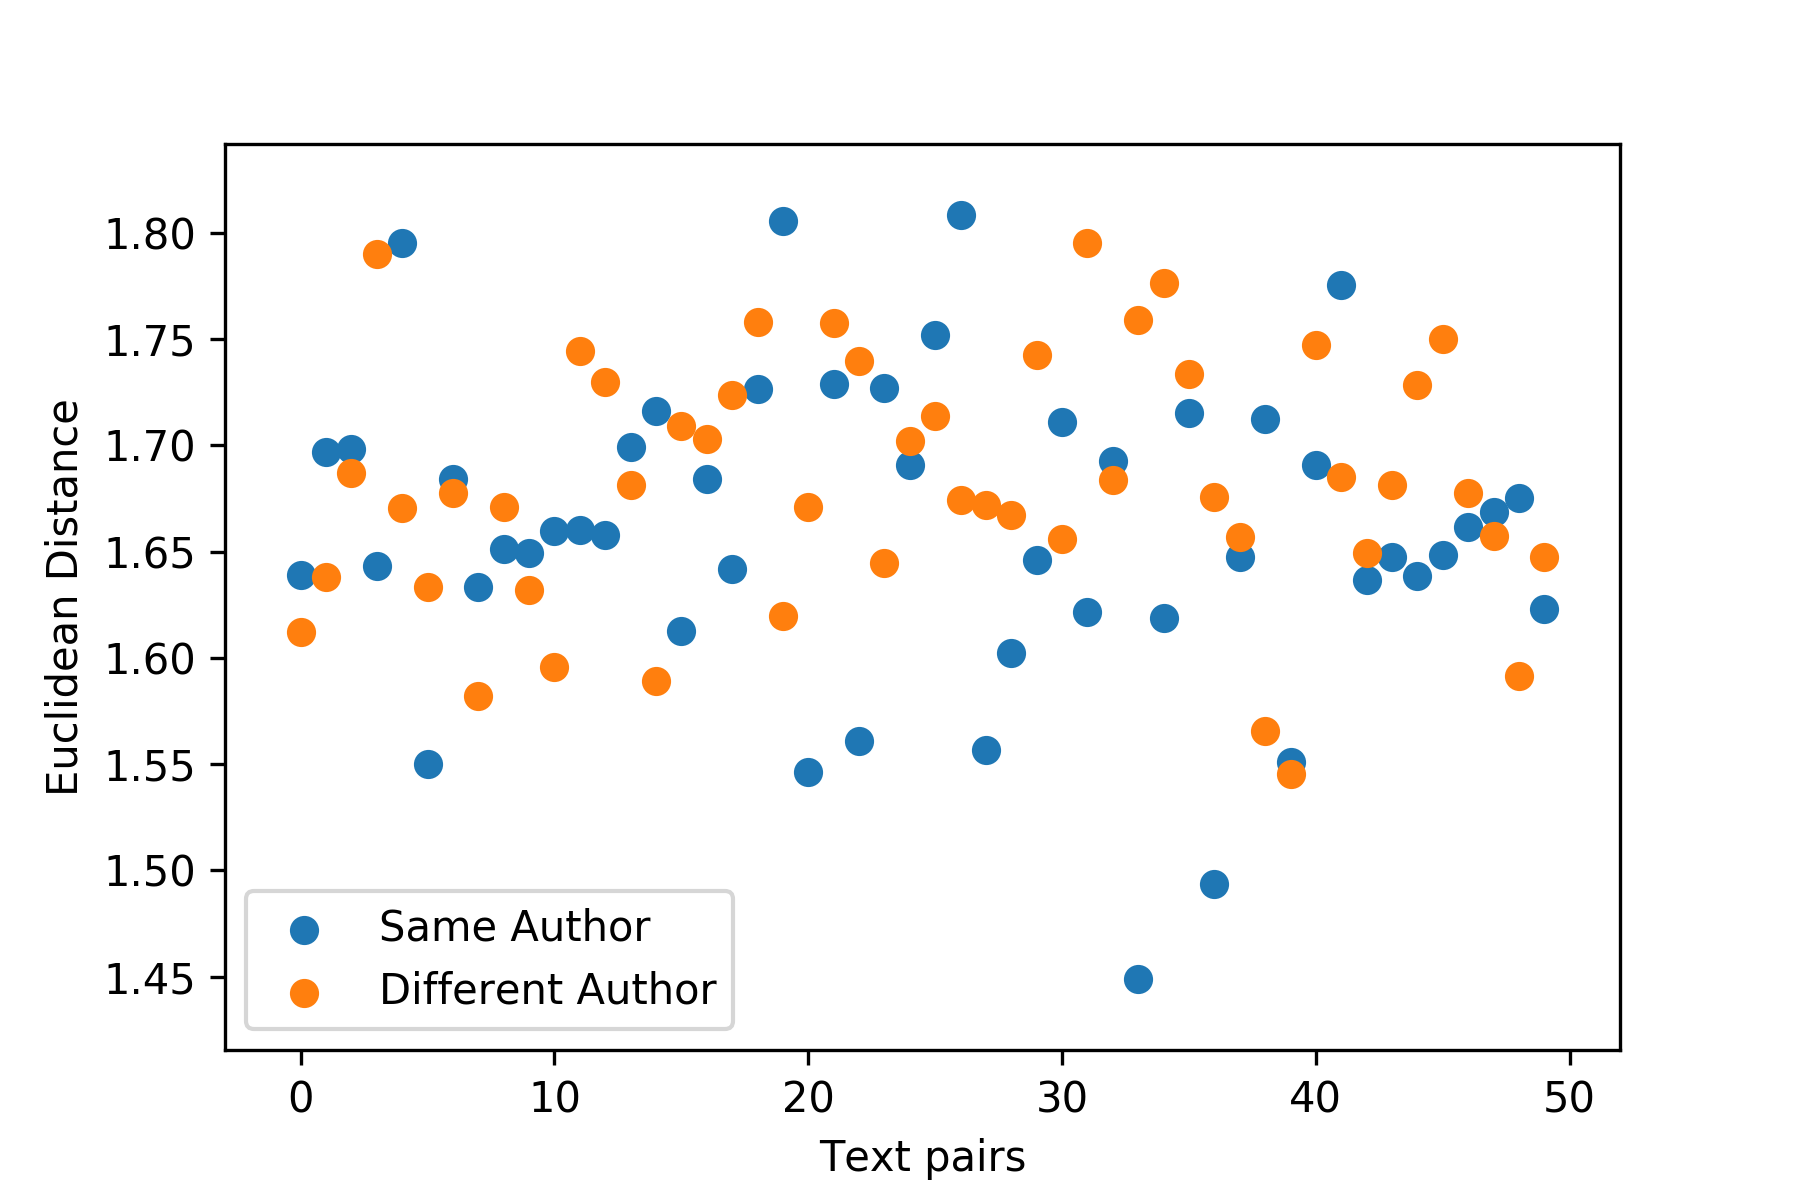
\includegraphics[width=\textwidth]{train_euc}
    \caption{The Euclidean distance between text-pairs for the training set (training on the test set).\label{fig:euc_train}}
  \end{minipage}
  \hfill
  \begin{minipage}[b]{0.49\textwidth}
    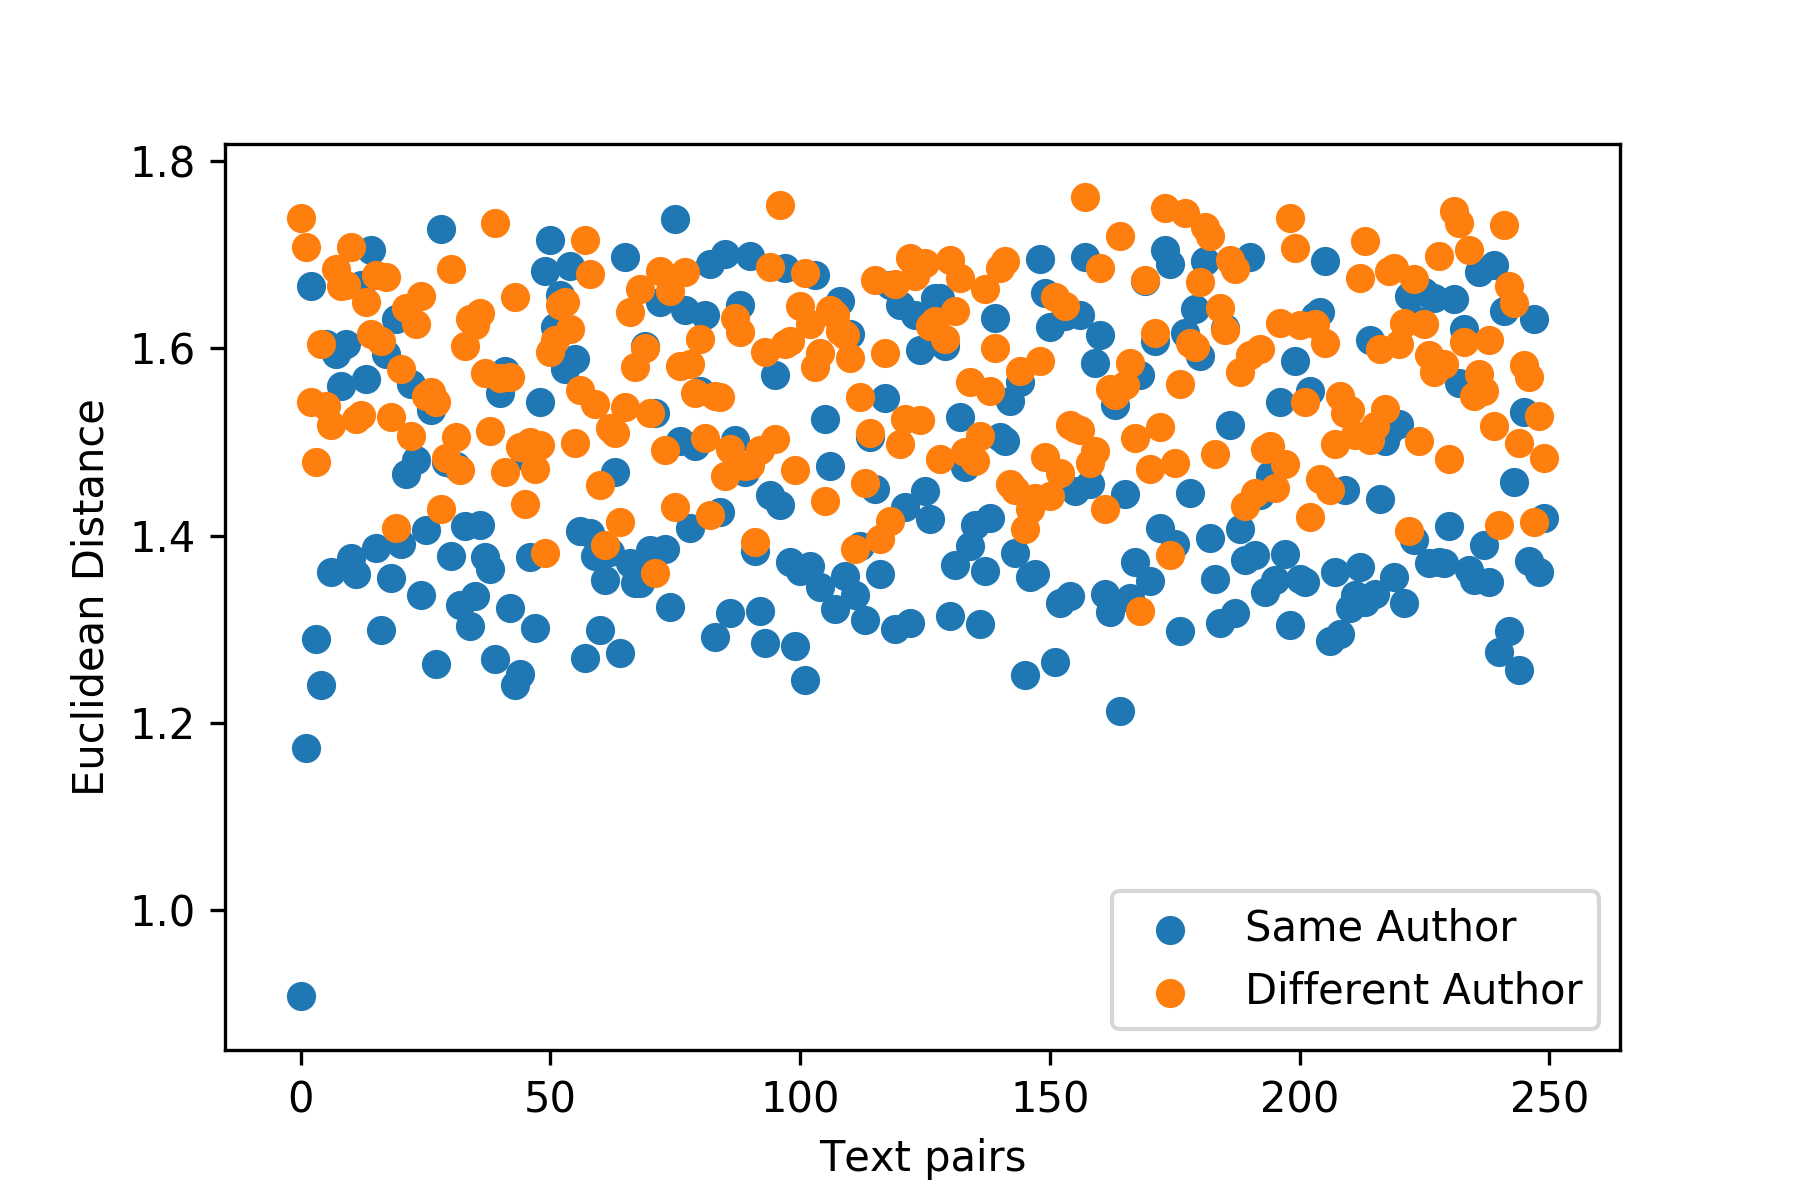
\includegraphics[width=\textwidth]{test_euc}
    \caption{The Euclidean distance between text-pairs for the test set (training on the training set)} \label{fig:euc_test}
  \end{minipage}
  \begin{minipage}[b]{0.49\textwidth}
    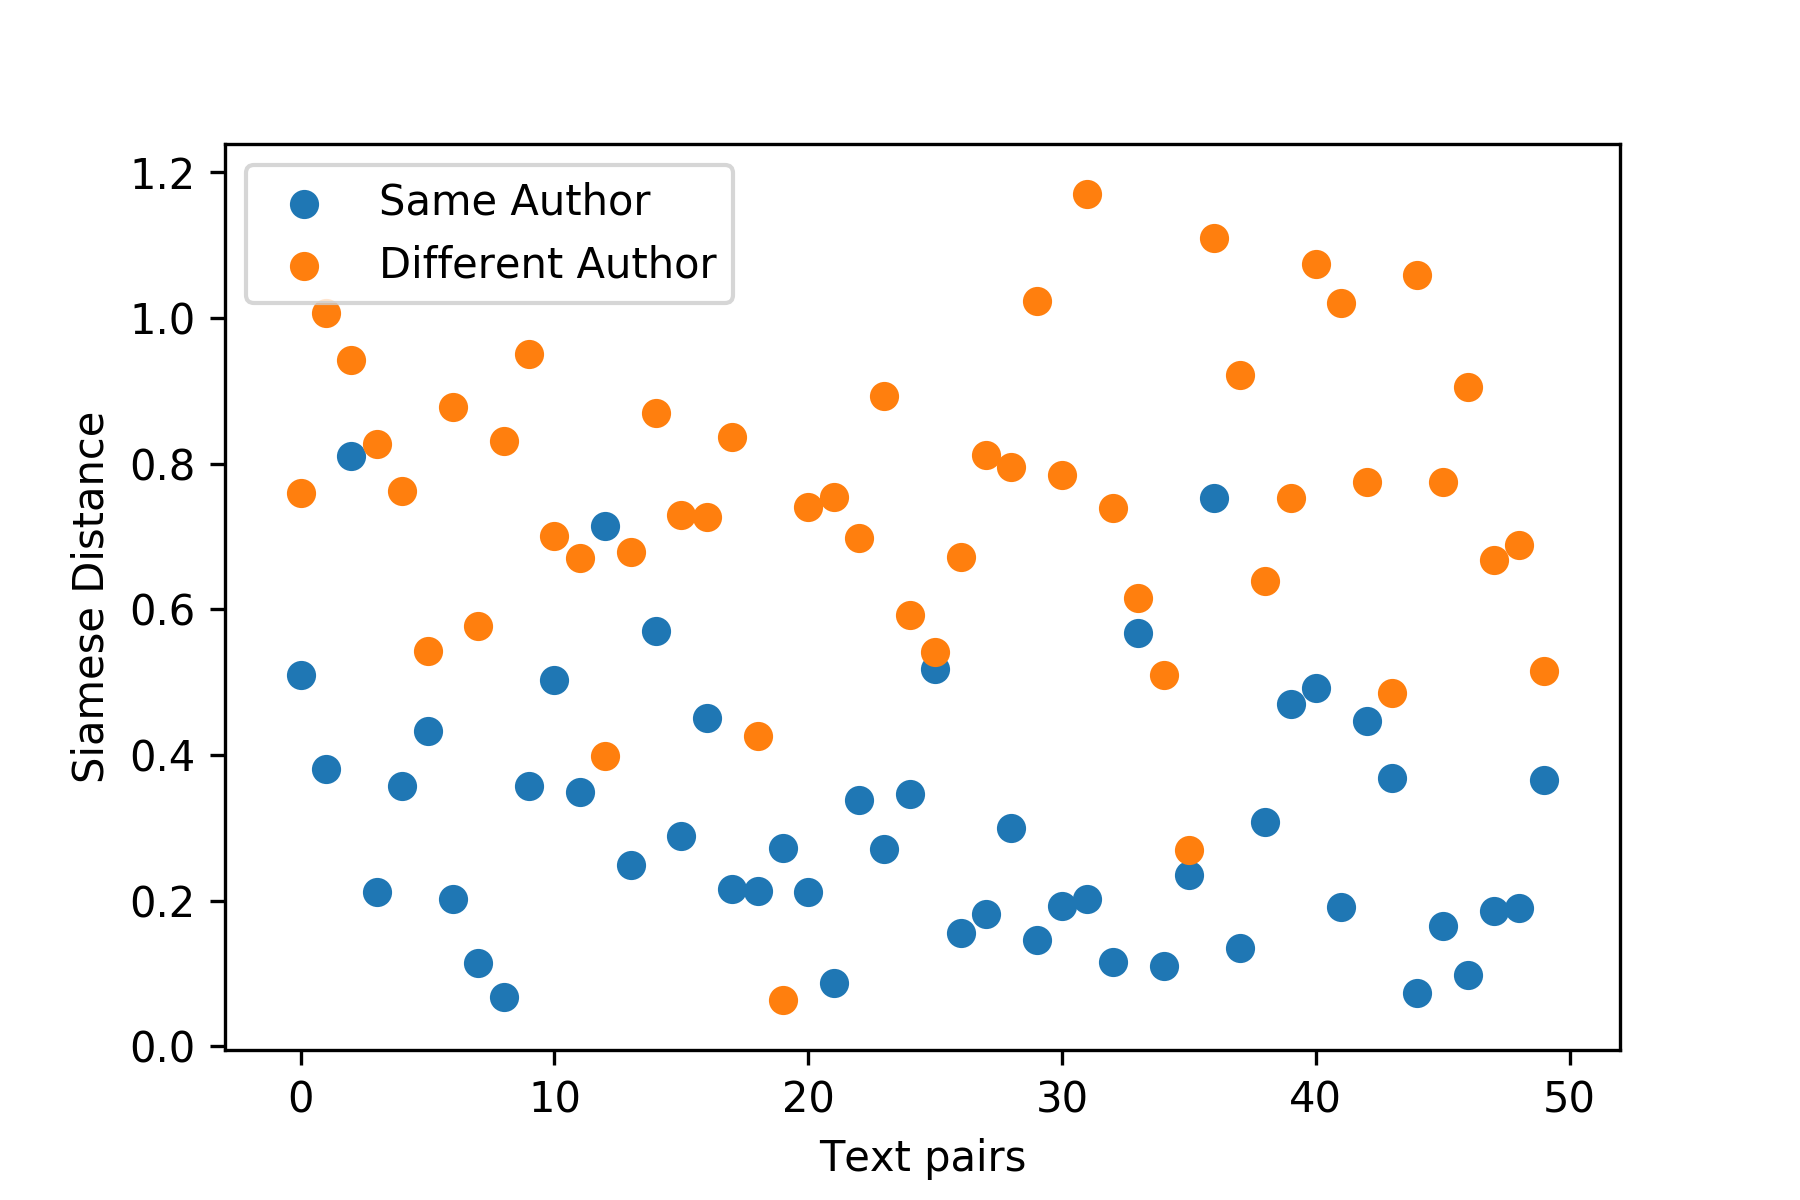
\includegraphics[width=\textwidth]{train_siam}
    \caption{The Siamese learned distance between text-pairs for the training set (training on the test set). \label{fig:siam_train}}
  \end{minipage}
  \hfill
  \begin{minipage}[b]{0.49\textwidth}
    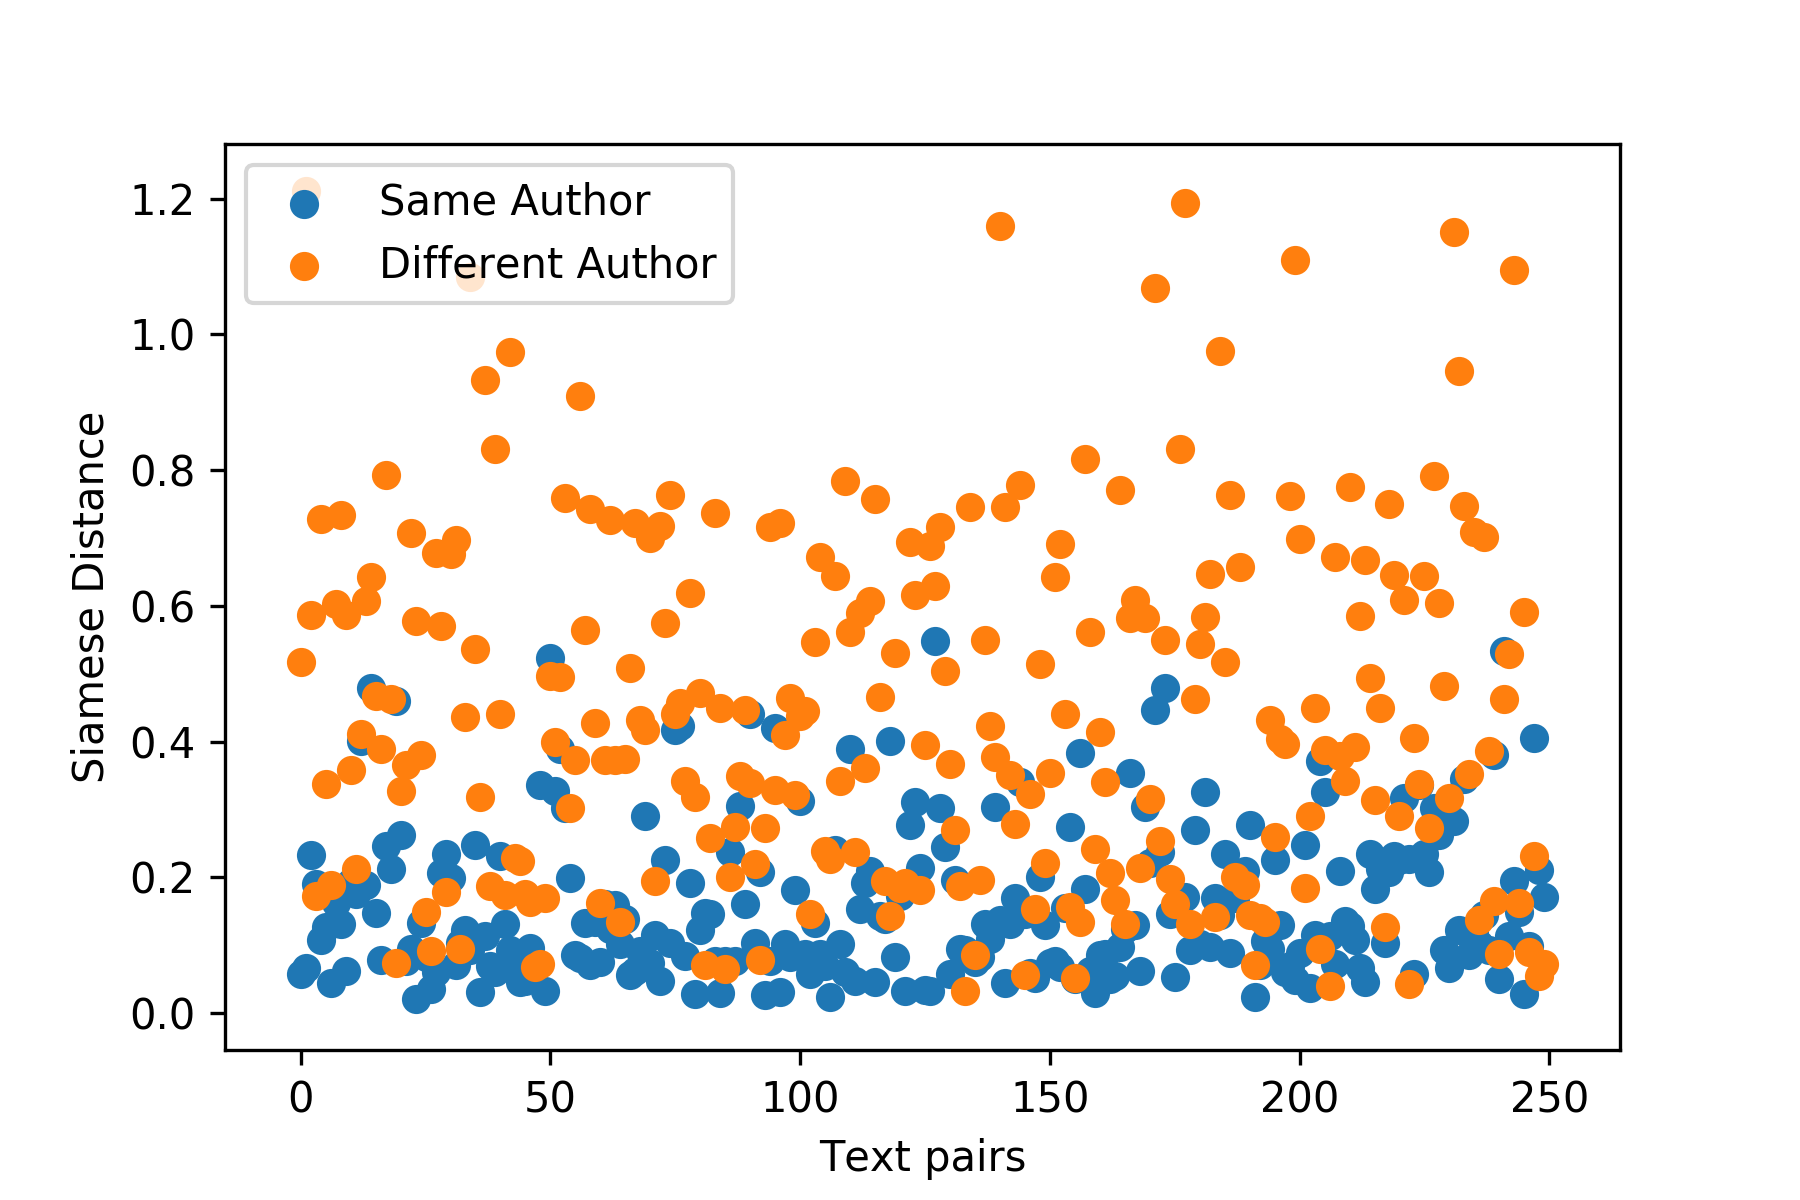
\includegraphics[width=\textwidth]{test_siam}
    \caption{The Siamese learned distance between text-pairs for the test set (training on the training set) \label{fig:siam_test}}
  \end{minipage}
\end{figure}


We present results on the other PAN datasets in Section \ref{res:siamese}.
